\section{Abstraction Techniques for Functional Verification}\label{sec:model}

One of the main challenges for the verification of concurrent software that we see is 
to automatically verify \emph{global functional} correctness properties of concurrent software. 
To reach this goal, we advocate an approach where a \emph{mathematical model} of a concurrent application is constructed, which provides an \emph{abstract view} of the program's behaviour, leaving out  details that are irrelevant for the properties being checked~\cite{BlomHZ15,OortwijnBGHZ17}, see Figure~\ref{fig:general}. The main verification steps in this approach are
\begin{enumerate}[topsep=0pt,noitemsep]
\item \emph{algorithmic verification} over the mathematical model to reason about global program behaviour, and 
\item \emph{program logics} to verify  the formal connection between the software and its mathematical model.
\end{enumerate} 

%\begin{wrapfigure}{o}{.25\textwidth}
\begin{figure*}[t]
\begin{center}
\fcolorbox{\leadingcolor}{White}{
\begin{tikzpicture}

\tikzset{
    depbox/.style={
      draw=\leadingcolor,
%      top color=white, bottom color=black!20,
      fill=lightgray,
      rounded corners, text badly centered},
    deparrow/.style={draw=black, dashed, shorten >=2pt, shorten <=2pt, ultra thick},
    connectarrow/.style={ultra thick,dashed,draw=\leadingcolor,shorten >=8pt, shorten <=8pt},
    wpbox/.style={
      fill=dblue!20!white,draw=black,text badly centered,inner sep=0pt,ellipse
    },     
    approxbox/.style={text width= 5cm
          },     
    featbox/.style={
          },     
}

\coordinate (topnode) at (0,5);
\coordinate (bottomnode) at (0, 1.5);
\coordinate (alinenode) at (-.5,1);
\coordinate (blinenode) at (.5, 1.5);

\node[inner sep=0pt] (abstraction) at (topnode)
  {\setlength{\fboxrule}{1pt}\fcolorbox{\leadingcolor}{\supportcolor}{
\includegraphics[width=2cm]{abstraction.pdf}}};    

\node[inner sep=0pt] (code) at (bottomnode)
 {\setlength{\fboxrule}{1pt}\fcolorbox{\leadingcolor}{\supportcolor}{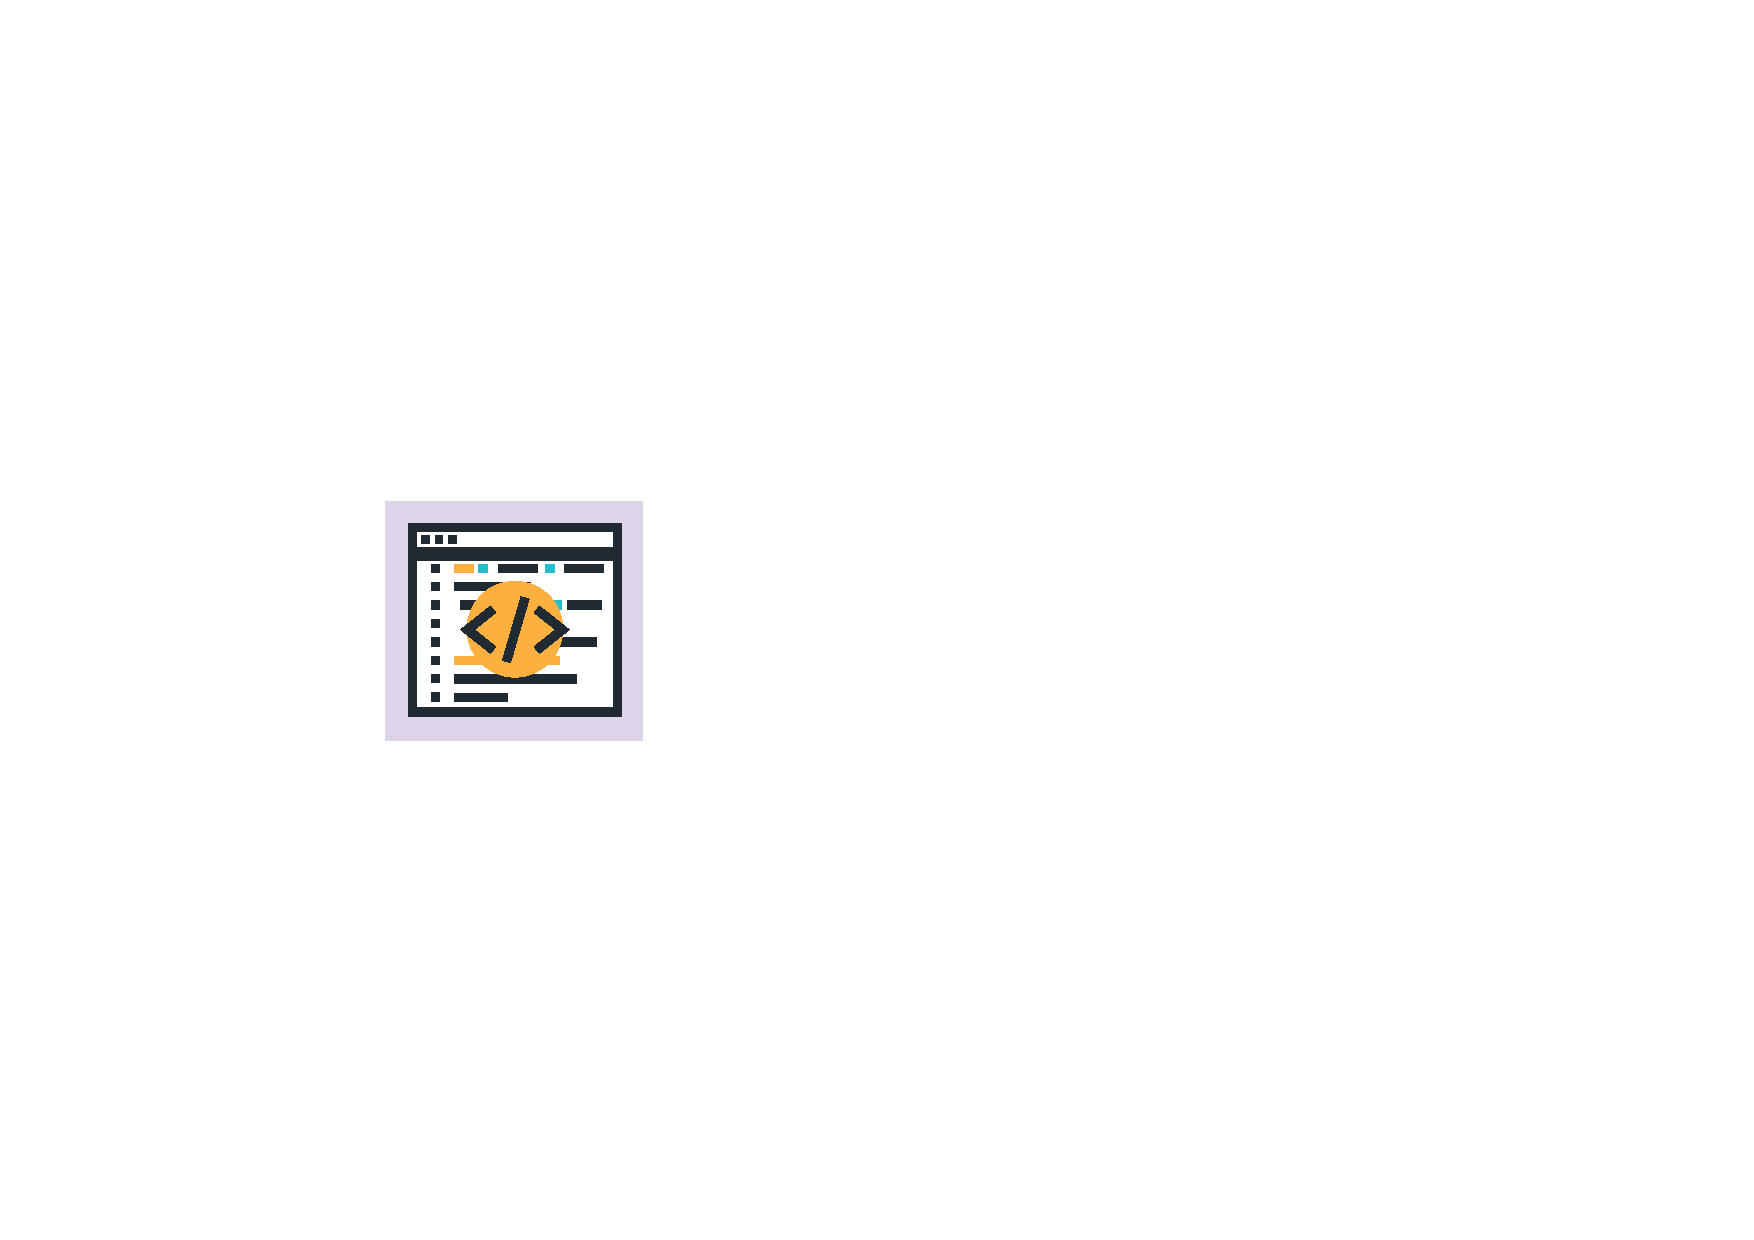
\includegraphics[width=2cm]{code.pdf}}};    

\draw[deparrow] (alinenode)--(-.5,5);
\draw[deparrow] (blinenode)--(.5,5.5);

\node[featbox] at (-1.2, 3.1){action \(a_1\)};
\node[featbox] at (1.3, 3.1){action \(a_2\)};
\node[featbox] at (2.6, 5){\quad{}Mathematical model};
\node[featbox] at (2.2, 1.5){\quad{}Software code};
\node[approxbox] at (7, 5){\textcolor{\leadingcolor}{Step 1: has property
  \(\phi_{\mathsf{abstract}}\) over actions \(a_1\) and \(a_2\)}};
\node[approxbox] at (7, 3.1){\textcolor{\leadingcolor}{Step 2: actions \(a_1\) and \(a_2\)
  correspond to suitable code fragments}};
\node[approxbox] at (7, 1.5){\textcolor{\leadingcolor}{Conclusion: code has property
  \(\phi_{\mathsf{concrete}}\)}};
% %\coordinate (designnode) at (0,-3);
% \coordinate (develnode) at (0,0);
% \coordinate (vcnode) at (4,0);
% \coordinate (vernode) at (8,0);
% % \coordinate (parnode) at (10,3);
% \coordinate (relnode) at (12,0);
% \coordinate (analysisnode) at (12,-3);
% \coordinate (cornernode) at (0,-3);

% %\node[depbox,fill=dblue!40!white,text width=2.5cm] (design) at (designnode) {\strut Design};
% \node[depbox,fill=dblue!40!white,text width=2.5cm] (devel) at
% (develnode) {\strut Design and\\Development};
% \node[depbox,fill=dblue!40!white,text width=2cm] (vc) at (vcnode) {\strut Service Integration};
% \node[depbox,fill=dblue!40!white, text width=2.5cm] (ver) at (vernode)
% {\strut Automated \\ Validation};
% % \node[depbox,text width=2.2cm] (par) at (parnode) {\strut Partial\\\strut Test Release};
% \node[depbox,fill=dblue!40!white, text width=3cm] (rel) at (relnode) {\strut
%   Release\\\strut (Trial or Global)};
% \node[depbox,fill=dblue!40!white, text width=2cm] (analysis) at (analysisnode) {\strut Problem\\\strut Analysis};

% % \draw[deparrow] (design.north) -- (devel.south);
% \draw[deparrow] (devel.east) -- (vc.west);
% \draw[deparrow] (vc.east) -- (ver.west);
% \draw[deparrow] (ver.east) -- (rel.west);
% % \draw[deparrow, shorten >=6pt, shorten <=6pt] (ver.north) -- (par.south);
% % \draw[deparrow, shorten >=6pt, shorten <=6pt] (par.south) -- (rel.north);
% \draw[deparrow] ([xshift=4mm]rel.south) -- ([xshift=4mm]analysis.north);
% \draw[deparrow, shorten >=6pt, shorten <=6pt] ([xshift=-2mm]analysis.north) -- ([xshift=-0mm]ver.south);
% \draw[deparrow,rounded corners] ([xshift=-0mm]analysis.west) -- (cornernode) --  ([xshift=-0mm]devel.south);

% % \node[wpbox,text width=1.8cm] (wp2) at ([yshift=-7mm]vc.south) {WP2:\\Differential\\Model};
% % \node[wpbox,text width=3.5cm] (wp34) at ([yshift=-4mm]ver.south)
% %   {WP3: Testing\\WP4: Static Analysis};

% % \node[wpbox,text width=3.5cm] (wp5) at (wp5node)
% %   {WP5: Validation\\and Integration};

% % \draw[connectarrow] (wp5.south)--(ver.north);
% % \draw[connectarrow] (wp5.south)--(vc.north);
% % \draw[connectarrow] (wp5.east)--(par.west);
% % \draw[connectarrow] (wp5.east)--(rel.north west);
% % \draw[connectarrow,bend left=30] (wp5.south east) to node{} ([xshift=4mm,yshift=-1mm]analysis.north west);

% % \node[featbox,text width=1.8cm] (em) at ([xshift=2mm,yshift=2mm]par.north east)
% %   {Evasive\\Monitoring};

% \node[featbox,text width=2.2cm,minimum size=2.5\baselineskip] (nem) at ([xshift=0mm,yshift=5mm]rel.north)
%   {Monitoring};

% \node[featbox,text width=2.8cm] at ([xshift=0mm,yshift=5mm]ver.north)
%   {\strut Dynamic/Static\\
%    Analysis};

% \node[featbox,text width=2.3cm] at ([xshift=0mm,yshift=5mm]vc.north)
%   {\strut Differential\\Model};


% % \node[featbox,text width=1.8cm] (customers) at ([xshift=8mm,yshift=0mm]rel.east)
% %   {1..\textasteriskcentered\\Customers};

% \node[featbox,text width=1.8cm] (time) at ([xshift=10mm,yshift=0mm]analysis.east)
%   {Error Analysis};
% % \node[featbox,text width=1.5cm] (model) at ([xshift=4mm,yshift=0mm]analysis.east)
% %   {Model};

% \node[above,inner sep=0pt] at ([xshift=-8mm,yshift=-0mm]$(cornernode) !.5! (analysis)$) {\strut Long Term Fix};

% \node[left,fill=white,inner sep=0pt] at ([xshift=-2mm,yshift=-2mm]$(ver) !.5! (analysis)$) {\strut Quick Fix};
% \node[right,inner sep=0pt] at ([xshift=5mm,yshift=-2mm]$(rel) !.5! (analysis)$) {\strut Problems};

\end{tikzpicture}
}
\end{center}
\caption{Using abstraction for the verification of concurrent and distributed software}\label{fig:general}
\end{figure*}
%\end{wrapfigure}


Typically, the basic building blocks of the abstract mathematical model are \emph{actions}, for which we can prove a correspondence between abstract actions and concrete code fragments.
%, which is then used to prove the formal connection between the software and its mathematical model. % Moreover, this has the advantage that if a global property does not hold at the abstract level, the abstract-level counterexample corresponds to a concrete candidate counterexample at the software level. 
A \emph{software designer} specifies the desired \emph{global properties} for a given application in terms of abstract actions. The \emph{software developer} then specifies how these \emph{abstract actions map to concrete program state}: in which states is the action allowed, and what will be its effect on the program state. Global properties may be safety properties, \emph{e.g.}, an invariant relation between the values of variables in different components, or a complicated protocol specifying correct interface usage, but we believe that extensions of the approach to liveness and progress properties are also possible. 
%This combination of the \emph{precision of program logics} with a provably correct and precise \emph{abstraction technique} enables \emph{automation} and \emph{scaling} of the verification of concurrent and distributed software, while keeping a high level of \emph{precision.}

To further develop this approach and make it scale, we believe the following challenges should be addressed:
\begin{enumerate}[topsep=0pt,noitemsep]
\item identify a good abstraction theory,
\item extend the abstraction theory to reason about progress and liveness properties of code, and 
\item use the abstraction theory to guide the programmer to develop working code through refinement.
\end{enumerate} 

% We discuss these challenges in more detail, and discuss our first results in this direction.

% \subsection{The Right Mathematical Model}
% The purpose of a good abstraction is that it reduces the verification effort in two ways:
% it makes it easier for the software designer to reason about the essential parts of his program, and automated verification methods can be used, because the verification effort is used on a model that is smaller than the original program. 
% Moreover, the abstraction should support modular and compositional verification.

% To find such a level of abstraction, we need to look at what currently hinders verification.
% One problem is the large state space of a program, as we have to consider all possible values of all program variables. 
% Thus, a suitable abstraction needs to be able to describe a reachable configuration of variables as a single mathematical object.
% %Considering modularity, this also means that reachable values for mathematical objects should be abstractable in the same way.

% Moreover, verification of concurrent software needs to consider all possible interleavings of the threads. Thus, we need to find ways to group actions, in particular also actions that do not occur inside atomic blocks of code. The theory of linearisation points will be a good starting point~\cite{Vafeiadis10,HemedRV15} for this, but it needs to be further generalised, as abstract actions also could correspond to method calls, and not just to memory writes.

% % Ideally, the modularity of a good abstraction can be used to make a good connection between the program code and some abstraction.
% % If the abstraction can be used to capture many properties about concrete code, its modularity can be used to abstract away from this.
% % The connection with the program is then obvious enough to be machine checkable on for the lowest level of abstraction.
% % On higher levels, the connection can be made entirely through exploiting the modularity of the abstraction technique.
% % This means that modularity should not mean that two models can be composed into a single one using some composition operation:
% % we need a form of modularity that allows us to abstract over the details of the underlying models, again reducing the number of variables and the number of interleavings that need to be reasoned about.


% Summarising, a good abstraction should have the following properties:
% \begin{itemize}[noitemsep=0pt,topsep=0pt]
% \item it can accurately capture low-level implementation details, 
% \item it is modular, 
% \item it can abstract over a sequence of multiple actions, and
% \item it can abstract over a valuation of multiple variables.
% \end{itemize}

% When developing this abstraction theory, we use the logics in the CSL family tree~\cite{BrookesO16} as an important source of inspiration. 
% In particular, the notion of views has been advocated as a general framework that captures many commonalities in the verification of concurrent software~\cite{DinsdaleBGPY13}, and we believe it is important that our basic abstraction theory can be described in terms of views.
% However, to further the state of the art in program verification, we believe there are two more additional requirements that should be considered, namely that the abstraction should be able to reason about time-dependent properties, and it should facilitate reasoning in a top-down manner, as will be motivated below.

% \subsection{Reasoning about Liveness and Progress.}
% Most of program verification concerns the verification of safety properties:
% functional correctness is interpreted as ensuring that under a certain precondition, the postcondition will hold after executing some code.
% Checking that a postcondition is not violated corresponds to verifying that variable assignments that violate the postcondition are not reachable, which is a safety property.
% However, when designing concurrent code, safety is only one issue software designers need to deal with, they also need to make sure that their program will not deadlock, and will eventually do the right thing.

% The latter property is called progress: if an action is enabled, it will eventually happen.
% Whether or not a progress property holds depends on a program scheduler, which depends on hardware, firmware, drivers and software.
% We therefore need an approach in which the assumptions about the scheduler can be made explicit.

% We wish to use the abstraction theory to support reasoning about global liveness properties.
% This means that the abstractions need to incorporate a notion that an action must happen.
% This has been explored earlier by Larsen \emph{et al.} who defined modal transition systems as an extension of standard LTSs with must- and may-transitions~\cite{LarsenT88,AntonikHLNW08}.

% Variant-based reasoning allows us to show that an action indeed will happen. As the actions might happen in different parts of the program, using this variant-based technique might not always be straightforward.
% We may develop a nested approach for variant-based reasoning, where at the lowest level we show that individual methods terminate, and at higher levels we show that a sequence of method calls terminates (assuming that the method calls themselves terminate).
% In the rewriting community there is a substantial amount of work on termination of rewrite systems, some of which has been applied to sequential programming languages and transition systems~\cite{Joosten16,Brockschmidt17,Giesl14}, and it should be investigated if and how these techniques can be used in the context of concurrent software verification. 

% \subsection{Unification of Model and Code}

% Finally, we believe that if the abstraction theory is fully developed, it should also be usable in 
% the opposite
% direction: if we take an abstract model as a starting point, can we
% use \emph{refinement} to transform this into correct working code?



% The basic refinement process can be divided into two phases. In the first phase, the global property can be separated into properties about individual processes. This might introduce some communication steps, and we need to resort here to the notion of process of equivalence under hiding of actions. The big challenge in this step is to decide how the property should be split. When verifying a concrete program, the program code dictates how this should be done. But in this case, where we wish to generate the program, we need other ways to do this. We plan to investigate different possibilities, for example maximising parallelisation, where each thread is responsible for an individual action, or even multiple threads execute the same action, all in parallel;  minimising parallelisation, and grouping sets of related actions. For all these possibilities, different splitting strategies can be developed, but typically some user intervention will be necessary here to indicate the intent of the program. 

% In the second phase, we have process algebra terms that describe the behaviour of an individual thread. The process algebra term itself describes the control flow of the thread, and we will develop a technique to transform each process algebra term into a sequence of program instructions. The abstraction typically defines some variables, which model the synchronisation between the different threads and are used to capture the effect of the actions. These variables should be mapped into concrete program variables, and as a last step the actions are translated into concrete program code, executing the action's specified effect. Typically, the guards will be fulfilled by construction, and do not have to be incorporated in the generated program code.

% In the long run, the results of these investigations might lead to a theory that unifies models and programs and removes the borders between the two. This would allow us to reason about systems where some components are already implemented, and others are only specified by a model, which later might be refined into an implementation. 


% \subsection{First Steps Towards a Solution}
% In our earlier work on abstract models~\cite{BlomHZ15,Zaharieva15,OortwijnBGHZ17VSTTE}, we have shown that it is possible to use process algebra terms to describe the abstract control flow of a program. This allow us to show that the program behaves according to a certain protocol (for example preventing unwanted flow of information by ensuring that a send may never occur after a receive) or that a variable evolves 
% according to a particular pattern (for example, a variable only increases, a queue never becomes empty etc.). The unique characteristic of this approach is that we can prove the correspondence between the abstract model and the program code using standard program logic, by linking the actions that are the basic building blocks of the model to concrete program statements. 

% Below, this approach is sketched on a very simple example. Suppose we have a shared variable \lstinline{x} protected by a lock \lstinline{lck}, and we have two threads that manipulate \lstinline{x}: one thread multiplies \lstinline{x} by 4, the other thread adds 4 to \lstinline{x}. The specification of the thread that performs the multiplication captures that the multiplication has happened. For this we use the notion of history~\cite{BlomHZ15}: an abstraction of the actions a thread has taken up-to now. If before the thread is executed, the history is equal to \emph{H} (written \emph{Hist(H)}), then afterwards the action \emph{mult(4)} is added at the end of the history (\(P.a\) is notation for a process \(P\), followed by action \(a\)). Similarly the specification of the addition thread captures that the addition has happened. The \emph{action} annotation inside the method body indicates the concrete code fragment that corresponds to this abstract action.


% \begin{lrbox}{\lstbox}
% \begin{minipage}{\textwidth - 6pt}
% \begin{lstlisting}[language=java,multicols=2,basicstyle=\small]
% class Mult extends Thread {

% //@ requires Hist(H);
% //@ ensures Hist(H.mult(4));
% public void run() {
%      //@ action mult(4) {
%        lock(lck); 
%        x = x * 4;
%        unlock(lck);
%      //@ } 
%   } 
% }
% class Add extends Thread {

% //@ requires Hist(H);
% //@ ensures Hist(H.add(4));
% public void run() {
%      //@ action add(4) {
%        lock(lck);
%        x = x + 4;
%        unlock(lck);
%      //@ } 
%   } 
% }
% \end{lstlisting}\ \vspace*{-.8em}
% \end{minipage}
% \end{lrbox}
% \vspace*{-.6em}
% \begin{center}
% \fcolorbox{\leadingcolor}{White}{\usebox\lstbox}
% \end{center}

% Next, we have action specifications that describe the effect of the actions \emph{mult} and \emph{add}. Using program logic, we can prove that the action implementations (in the thread bodies) indeed behave as specified. 

% \begin{lrbox}{\lstbox}
% \begin{minipage}{\textwidth - 6pt}
% \begin{lstlisting}[language=java,basicstyle=\small]
% //@ assume true;
% //@ guarantee x == \old(x) * k;
% action mult(k);

% //@ assume true;
% //@ guarantee x == \old(x) + k;
% action add(k);
%  \end{lstlisting}\ \vspace*{-.8em}
% \end{minipage}
% \end{lrbox}
% \begin{center}
% \fcolorbox{\leadingcolor}{White}{\usebox\lstbox}
% \end{center}

% Suppose we have a \lstinline{main} method, which starts the two threads and then waits for them to terminate. For this main method we can specify and verify (using a history-aware program logic) that it will execute the \emph{mult} and the \emph{add} action in any order (where \(P + Q\) denotes a non-deterministic choice between \(P\) and \(Q\) and \emph{empty} denotes an empty history). 

% \begin{lrbox}{\lstbox}
% \begin{minipage}{\textwidth - 6pt}
% \begin{lstlisting}[language=java,basicstyle=\small]
% //@ requires Hist(empty) & x == 0;
% //@ ensures Hist(mult(4).add(4) + add(4).mult(4));
% public void main(...) {
%   Thread t1 = new Mult();  Thread t2 = new Add();
%   t1.fork(); t2.fork();
%   t1.join(); t2.join();
% }
%  \end{lstlisting}\ \vspace*{-.8em}
% \end{minipage}
% \end{lrbox}
% \begin{center}
% \fcolorbox{\leadingcolor}{White}{\usebox\lstbox}
% \end{center}

% From the history specification of the \lstinline{main} method and the action specifications, we can derive the possible values of variable x after termination of the \lstinline+main+ method, \emph{i.e.}, x can be either 4 or 16. 

% This example is very simple, but the same approach can be used in many different settings: for larger programs, non-terminating programs, distributed programs etc. In particular, for non-terminating programs, an abstraction can be used to predict the (abstract) behaviour, and correctness of the abstraction boils down to showing that the program flow never moves out of the predicted behaviour~\cite{Zaharieva15,OortwijnBGHZ17VSTTE}. We have used this approach to prove properties such as:  in a concurrent queue, the order of elements is preserved~\cite{AmighiBH16}; adherence to protocols that are commonly used to capture essential security properties, such as `no send after receive'~\cite{OortwijnBGHZ17VSTTE}; and correctness of an active object implementation using MPI operations~\cite{Zeilstra16}. Our own VerCors tool set provides support to reason in this way, but also the VeriFast tool can reason about histories (personal communication by Bart Jacobs, KU Leuven).

%  Note that an essential difference with other existing abstraction-based approaches such as CEGAR and IC3~\cite{Bradley11,ClarkeGJLV00,MalkisPR10} is how the correctness of the abstraction is proven. Usually, the relation between the original program and the abstract program is proven as a meta-theorem, and one has to trust the implementation of the algorithm that performs the abstractions (or check it manually), while in our approach the program logic is used to prove correctness of the abstraction. 

% % We will investigate if histories and futures also can be incorporated in this framework, as it might facilitate combinations with other logics.


\section{Automating the Verification Process}\label{sec:automation}

Another major challenge is how to automate the verification process.
At the moment, program verification requires many user annotations, explicitly describing properties which are often obvious to developers. We believe that many of the required annotations can be generated automatically, using a combination of appropriate static analyses and smart heuristics. 

We  advocate a very pragmatic approach to annotation generation, where any technique that can be used to reduce the annotation burden is applied, combined with a smart algorithm to evaluate the usability of a generated annotation, removing any annotations that do not help automation.  This will lead to a framework where for a large subset of non-trivial programs, we can automatically verify many common safety properties (absence of null-pointer dereferencing, absence of array out of bounds indexing, absence of data races etc.), and if we wish to verify more advanced functional properties, the developer might have to provide a few crucial annotations, but does not have to spell out in detail what happens at every point in the program (in contrast to current program verification practice). 

%However, it should be stressed that with this approach, we will never be able to automatically verify correctness of all programs; there will always be programs using unusual patterns, which need additional manual annotations in order to be verified.

% We believe that efficient annotation generation should build on existing static analyses and heuristics~\cite{FM12,GaleottiFMFZ15,Janota07,DohrauSUMM18} extended with tailor-made new generation techniques, aiming for an optimal verification result within a minimal amount of time. 

% There is a plethora of tools and techniques available which can be used to derive properties about the program state. However, many of these tools work on simple idealised languages, and these results will have to be extended to a more realistic programming setting. In particular, some approaches do not consider aliasing, which is often essential for the correctness of a program. 

% Moreover, if we use any technique that is available, this might lead to an overload of annotations, which can have a negative impact on verifiability. We thus need to find an optimal balance in how and when to generate annotations automatically. This will be an incremental process, where we use different analyses or heuristics to generate annotations and then select those that help towards our goal. Some of the generated annotations will need other auxiliary annotations to be verified automatically, thus we need to find a suitable order in which to apply the annotation generation algorithms. For example, if an analysis is sensitive to aliasing, we might first want to use an analysis which can derive some annotations about when two variables may or may not be aliased. Note that if we use unsound heuristics to generate annotations, this may lead to conflicting annotations, which might actually give a false impression of program correctness. Therefore, we also need to investigate efficient ways to avoid conflicting annotations. In some cases, a syntactic check will be sufficient to conclude that two annotations are not conflicting. Making optimal use of these cases will help to make this conflict check efficient.

% Lastly, if an annotation cannot be verified, we have to investigate how to provide the most suitable feedback. It is important to distinguish between the two following cases:
% \begin{enumerate}[topsep=0pt,noitemsep]
% \item a counterexample exists, which thus means that the annotation is incorrect. In this case, either the annotation is removed, or if a counterexample exists for the property the developer wanted to show for the program, the counterexample has to be presented to the user. In that case, it is important that the counterexample is intelligible, and helps the developer to understand why the program does not have the intended behaviour, and how to fix this.
% \item there is not sufficient information to prove the annotation. In this case, the annotation might still be kept as a candidate annotation, because when more annotations are generated, it might become possible to prove it. An intelligent strategy will be needed to keep potentially interesting annotations (for example, if the annotation would help to prove the globally desired property, it is potentially interesting), while ignoring others. 
% \end{enumerate}



\section{Verification of Programs using Different Concurrency Paradigms}\label{sec:other}
Finally, verification techniques need to support different programming languages, and different concurrency paradigms. 
% Most work on the verification of concurrent software focuses on shared memory concurrency with heterogeneous threading, as can be found, \emph{e.g.}, in Java or C. In this model, all threads have access to a shared memory, and all threads execute their own program code. However, in practice there are many other concurrency models in use (and there is also more and more hardware that supports these concurrency models directly). Therefore, we need to investigate how our verification approaches can be used for these other concurrency models as well. 
In particular, we believe that it is important to investigate how to reason about programs written using the structured parallel programming model where all threads execute the same instructions. Recently, we have shown how our verification techniques can be adapted in a straightforward manner to GPUs (including atomic update instructions)~\cite{BlomHM14,BlomDH15}. 
%On GPUs, there is a shared memory, but all threads execute the same program instructions (but operate on a disjoint part of the memory). 
It  turns out that the restricted setting of a GPU has a positive impact on verification: the same verification techniques can be used, and verification actually gets simpler.
% Because of the simpler concurrency paradigm, reasoning about many functional properties can be done without the need for abstraction, because the behaviour of all the other threads is more predictable. However, to reason about the interaction of the vector program in interaction with the host program, which invokes the vector program (the kernel), we are again back to the heterogeneous setting, and the abstraction theory can be used to give an abstract specification of the behaviour of the vector program.
We believe that this direction should be explored further, as typical GPU programs are usually quite low-level, which makes them more error-prone. %Thus, there is a high need to further develop automated techniques to reason about such applications. 

%It is also interesting to look at how these programs are developed. 
% One commonly-used approach is that a developer writes a sequential program and gives compiler hints about possible parallelisations~\cite{BaghdadiCGVIGKKLNWD13}. When this approach is used, a programmer is greatly helped by automated verification of these compiler directives. For basic compiler directives, we developed  verification techniques to prove the correctness of these parallelisations, \emph{i.e.}, to prove that if the program is parallelised, its behaviour will be equivalent to the behaviour of the sequential program~\cite{BlomDH15,DarabiBH17}, but this approach is still in its early stages, and needs to be developed further, allowing for more advanced compilation patterns. 

An interesting extension of this work is to automatically transform a verified sequential program with annotations into an annotated GPU program, which will be directly verifiable~\cite{HuismanBDS18}.
We believe this idea can also be used for other compiler optimisations, such that
 % For example, vector programs written in OpenCL (a platform-independent programming language for GPUs) can be executed both on CPUs and GPUs, but experiments have shown that to optimise performance, the data format should be different~\cite{Shen15}.
they do transform  not only the program, but also the correctness annotations, such that the result is a (hopefully) verifiable program again. Instead of proving correctness of the transformation, both the program and the annotations are transformed, such that after the transformation the resulting program with annotations can be reverified.

% Another interesting paradigm that deserves more attention is the area of distributed software, where we need techniques to 
% reason about programs without shared memory. One particular instance of these are distributed programs, but there are also concurrency paradigms, such as the message-box concurrency model of Scala, where each parallel computation works on its own memory. We have shown that 
% reasoning about distributed programs using the message passing interface (MPI) builds on the same principles~\cite{FuturePlaces} as reasoning about shared memory concurrency, but here the abstraction plays an even more important role, because it models the communication between the different computations. By adding a notion of synchronisation to the actions, we can model the communication. By defining variations in the action synchronisation, it should be possible to model other distributed programming models, such as the actor model, as well as the Scala concurrency model (on a single computer, with instantaneous send and receive), or variations of the MPI model, where the sending of messages can take time, and messages can bypass each other. It would even be possible to use this kind of reasoning at a lower level, for example to prove the correctness of an MPI implementation, where we take into account that messages might be lost.





